%%%%%%%%%%%%%%%%%%%%%%%%%%%%%%%%%%%%%%%%%
% Short Sectioned Assignment LaTeX Template Version 1.0 (5/5/12)
% This template has been downloaded from: http://www.LaTeXTemplates.com
% Original author:  Frits Wenneker (http://www.howtotex.com)
% License: CC BY-NC-SA 3.0 (http://creativecommons.org/licenses/by-nc-sa/3.0/)
%%%%%%%%%%%%%%%%%%%%%%%%%%%%%%%%%%%%%%%%%

%----------------------------------------------------------------------------------------
%	PACKAGES AND OTHER DOCUMENT CONFIGURATIONS
%----------------------------------------------------------------------------------------

\documentclass[paper=a4, fontsize=10pt]{article} % A4 paper and 11pt font size


\usepackage[vmargin=2.5cm,hmargin=3cm]{geometry}
% ---- Entrada y salida de texto -----

\usepackage[T1]{fontenc} % Use 8-bit encoding that has 256 glyphs
\usepackage[utf8]{inputenc}
\usepackage{helvet}
\renewcommand{\familydefault}{\sfdefault}
%\usepackage{fourier} % Use the Adobe Utopia font for the document - comment this line to return to the LaTeX default

% ---- Idioma --------

\usepackage[spanish, es-tabla]{babel} % Selecciona el español para palabras introducidas automáticamente, p.ej. "septiembre" en la fecha y especifica que se use la palabra Tabla en vez de Cuadro

% ---- Otros paquetes ----
\usepackage[hidelinks]{hyperref} % Estilo para los enlaces
\hypersetup{
  colorlinks   = true, %Colours links instead of ugly boxes
  urlcolor     = blue, %Colour for external hyperlinks
  linkcolor    = black, %Colour of internal links
  citecolor   = blue %Colour of citations
}
\usepackage{url} % ,href} %para incluir URLs e hipervínculos dentro del texto (aunque hay que instalar href)
\usepackage{amsmath,amsfonts,amsthm} % Math packages
%\usepackage{graphics,graphicx, floatrow} %para incluir imágenes y notas en las imágenes
\usepackage{graphics,graphicx, float} %para incluir imágenes y colocarlas

%Para incluir codigo
\usepackage{minted}

% Para hacer tablas comlejas
%\usepackage{multirow}
%\usepackage{threeparttable}

%\usepackage{sectsty} % Allows customizing section commands
%\allsectionsfont{\centering \normalfont\scshape} % Make all sections centered, the default font and small caps

\usepackage{fancyhdr} % Custom headers and footers
\pagestyle{fancyplain} % Makes all pages in the document conform to the custom headers and footers
\fancyhead{} % No page header - if you want one, create it in the same way as the footers below
\fancyfoot[L]{} % Empty left footer
\fancyfoot[C]{} % Empty center footer
\fancyfoot[R]{\thepage} % Page numbering for right footer
\renewcommand{\headrulewidth}{0pt} % Remove header underlines
\renewcommand{\footrulewidth}{0pt} % Remove footer underlines
\setlength{\headheight}{13.6pt} % Customize the height of the header

\numberwithin{equation}{section} % Number equations within sections (i.e. 1.1, 1.2, 2.1, 2.2 instead of 1, 2, 3, 4)
\numberwithin{figure}{section} % Number figures within sections (i.e. 1.1, 1.2, 2.1, 2.2 instead of 1, 2, 3, 4)
\numberwithin{table}{section} % Number tables within sections (i.e. 1.1, 1.2, 2.1, 2.2 instead of 1, 2, 3, 4)

\setlength\parindent{0pt} % Removes all indentation from paragraphs - comment this line for an assignment with lots of text

\newcommand{\horrule}[1]{\rule{\linewidth}{#1}} % Create horizontal rule command with 1 argument of height


%----------------------------------------------------------------------------------------
%	TÍTULO Y DATOS DEL ALUMNO
%----------------------------------------------------------------------------------------

\title{	
\normalfont \normalsize 
\textsc{\textbf{Ingeniería de Servidores (2016-2017)} \\ Grado en Ingeniería Informática \\ Universidad de Granada} \\ [25pt] % Your university, school and/or department name(s)
\horrule{0.5pt} \\[0.4cm] % Thin top horizontal rule
\huge Memoria Práctica 3 \\ % The assignment title
\horrule{2pt} \\[0.5cm] % Thick bottom horizontal rule
}

\author{Jose Luis Martínez Ortiz} % Nombre y apellidos

\date{\normalsize\today} % Incluye la fecha actual

%----------------------------------------------------------------------------------------
% DOCUMENTO
%----------------------------------------------------------------------------------------

\begin{document}

\maketitle % Muestra el Título

\newpage %inserta un salto de página

\tableofcontents % para generar el índice de contenidos

\listoffigures

\listoftables

\newpage

%\textbf{NOTA: en caso de problema al compilar, compruebe que tiene el paquete: texlive-babel-spanish.noarch }  \\
 
\newpage

%----------------------------------------------------------------------------------------
%	Cuestión 1
%----------------------------------------------------------------------------------------

\section{Cuestión 1:}
\subsection{a) ¿Qué archivo le permite ver qué programas se han instalado con el gestor de paquetes?}
En CentOS es el archivo \texttt{/var/log/yum.log}, en Ubuntu esta en \texttt{/var/log/apt/history.log}.


\subsection{b) ¿Qué significan las terminaciones .1.gz o .2.gz de los archivos en ese directorio?}
Significan archivos anteriores de log. Los ficheros de log crecen muy rápido y necesitan almacenarse
ahorrando el máximo espacio posible, para ello hay una configuración que indica cuanto tamaño debe de
tener el fichero de log y cuando excede ese tamaño se comprime en un fichero <log>X.gz siendo X el número
que identifica a los logs antiguos.



%----------------------------------------------------------------------------------------
%	Cuestión 2
%----------------------------------------------------------------------------------------

\section{Cuestión 2: ¿qué archivo ha de modificar para programar una tarea? Escriba la línea necesaria para ejecutar una vez al día una copia del directorio ~/codigo a ~/seguridad/\$fecha donde \$fecha es la fecha actual (puede usar el comando date).}
Para programar una tarea hay que modificar el archivo de configuración del \textit{/etc/crontab},
pero se recomienda realizar todas las modificaciones mediante el comando ``\textit{crontab -e}''.
Lo ideal es utilizar un script para la nueva tarea, para ello creo el script y lo pruebo como
se aprecia en la figura \ref{fig:P3_2_1}, después de la comprobación borro los ficheros copiados. \\
Ahora vamos a utilizar el comando \textit{crontab -e} para añadir al cron la nueva tarea
como se ve en la figura \ref{fig:P3_2_3}. Aplico que se ejecute cada día del mes de todos los meses
de todos los años a las 18:38 horas, elijo esta hora para no esperar mucho la comprobación.
En la figura \ref{fig:P3_2_2} se puede ver como ha funcionado correctamente.

\begin{figure}[H] %con el [H] le obligamos a situar aquí la figura
\centering
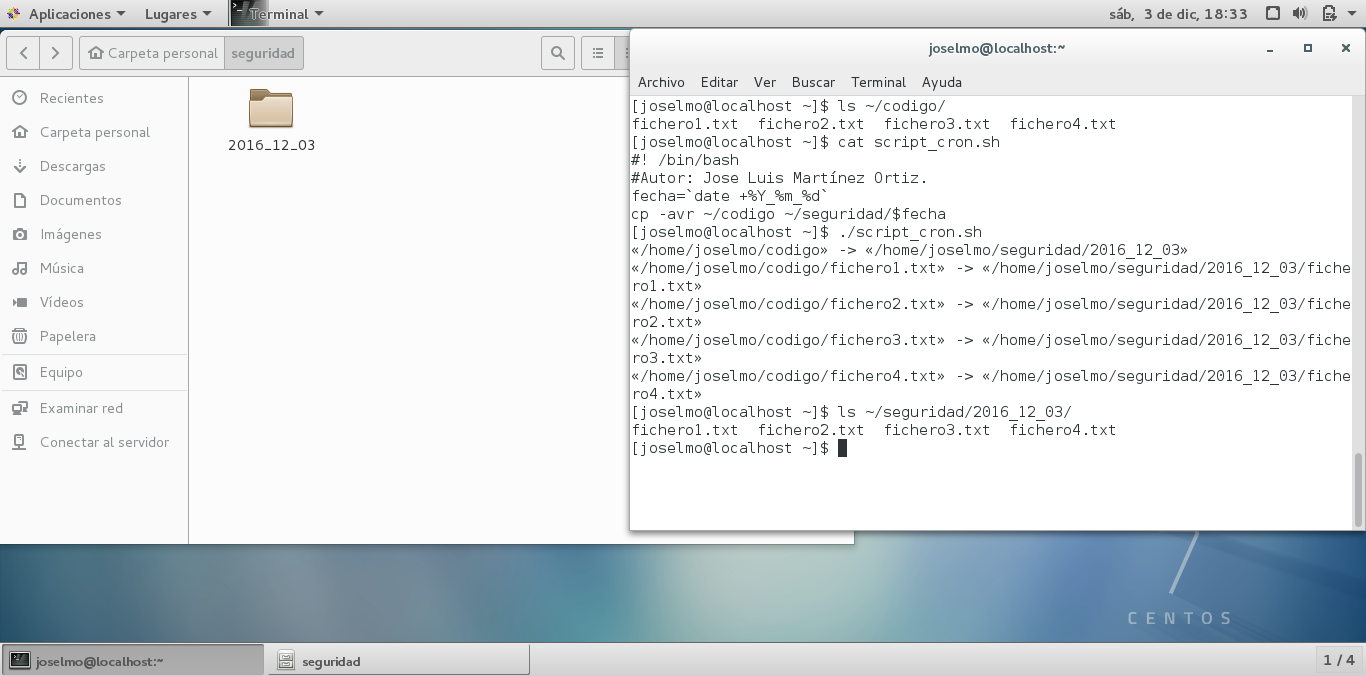
\includegraphics[scale=0.4]{./imagenes/P3_2_1.png} 
\caption{Script para copiar un directorio en otro con la fecha actual} \label{fig:P3_2_1}
\end{figure}

\begin{figure}[H] %con el [H] le obligamos a situar aquí la figura
\centering
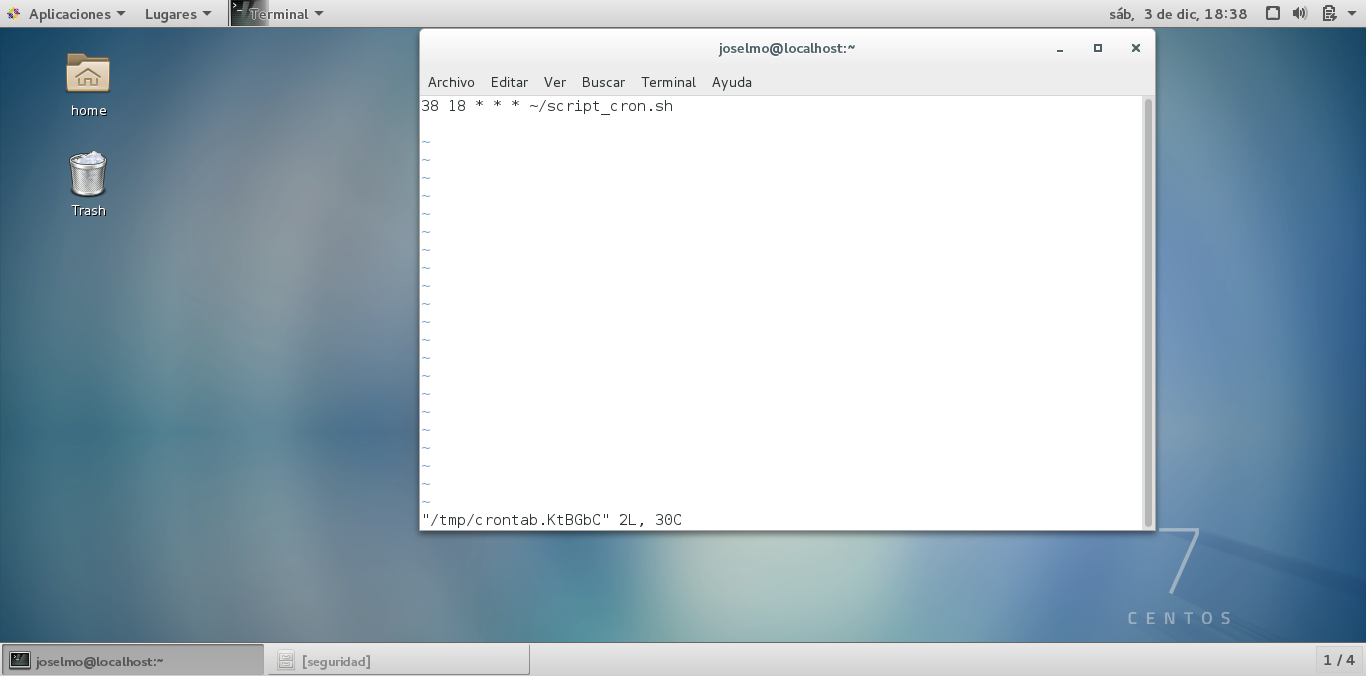
\includegraphics[scale=0.4]{./imagenes/P3_2_3.png} 
\caption{Edición del fichero /etc/crontab mediante el comando \textit{crontab -e}} \label{fig:P3_2_3}
\end{figure}

\begin{figure}[H] %con el [H] le obligamos a situar aquí la figura
\centering
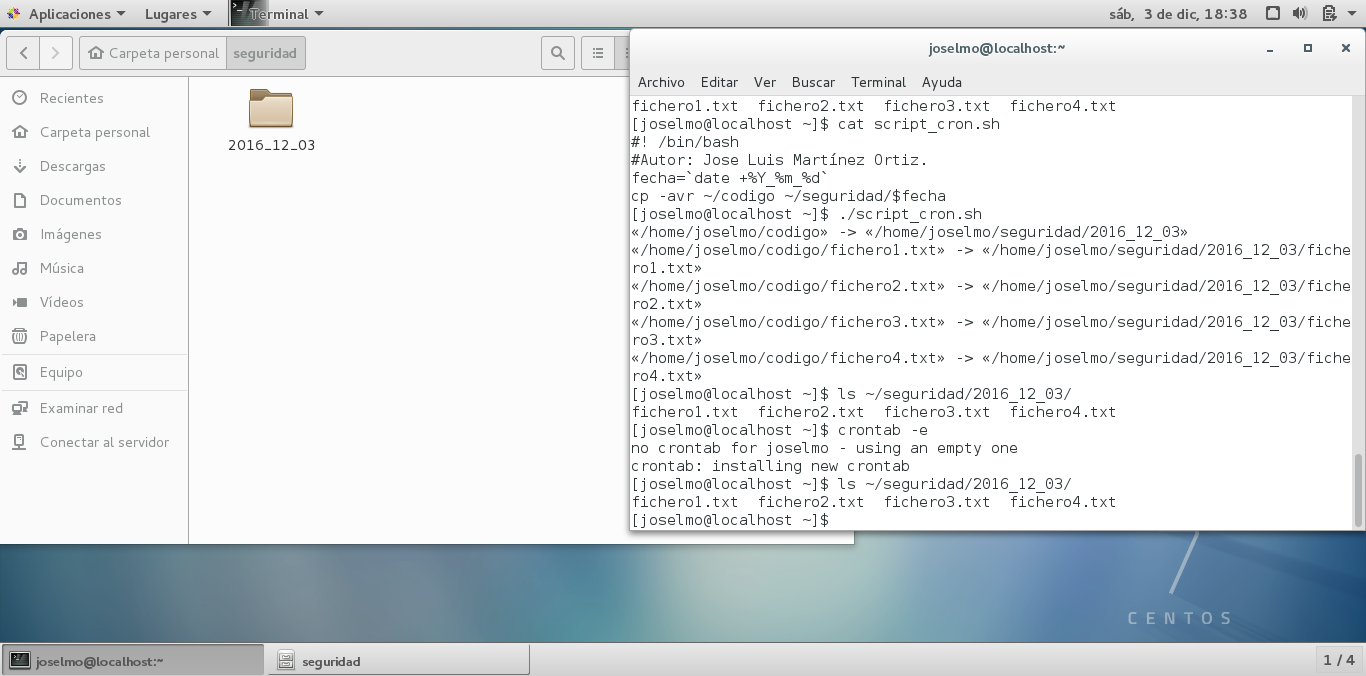
\includegraphics[scale=0.4]{./imagenes/P3_2_2.png} 
\caption{Resultado de la tarea nueva del cron} \label{fig:P3_2_2}
\end{figure}

%----------------------------------------------------------------------------------------
%	Cuestión 3
%----------------------------------------------------------------------------------------

\section{Cuestión 3: Pruebe a ejecutar el comando, conectar un dispositivo USB y vuelva a ejecutar el comando. Copie y pegue la salida del comando. (considere usar dmesg | tail). Comente qué observa en la información mostrada.}
En mi caso utilizo la web cam de VirtualBox ya que el pen drive no me lo reconoce, aun instalando
el \textit{extension pack}.
Como se puede ver en la figura \ref{fig:P3_3_1}, se ha registrado la conexión de un dispositivo por
un puerto USB, indicando datos de la Web cam como el fabricante, número de serie, el driver que 
es necesario para utilizar el dispositivo, detectando que es una entrada de vídeo incluso.

\begin{figure}[H] %con el [H] le obligamos a situar aquí la figura
\centering
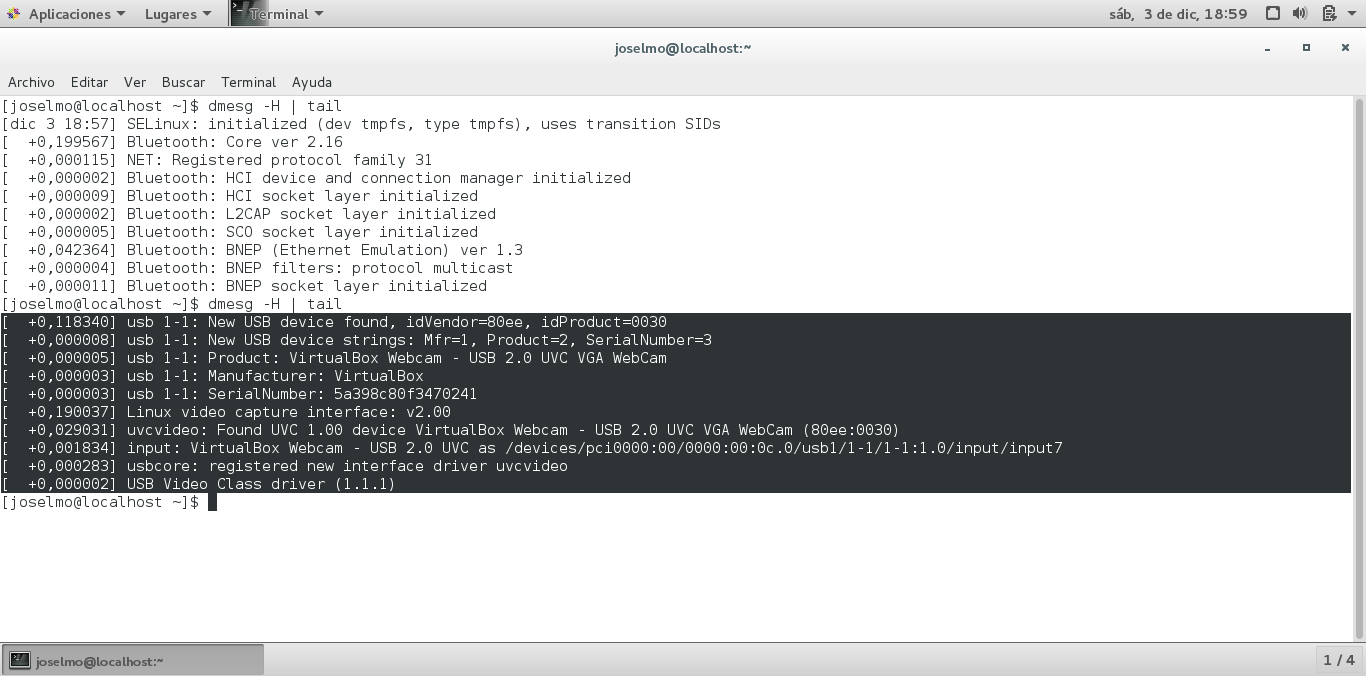
\includegraphics[scale=0.4]{./imagenes/P3_3_1.png} 
\caption{Resultado dmesg al conectar una web cam} \label{fig:P3_3_1}
\end{figure}

%----------------------------------------------------------------------------------------
%	Cuestión 4
%----------------------------------------------------------------------------------------

\section{Cuestión 4: Ejecute el monitor de “System Performance” y muestre el resultado. Incluya capturas de pantalla comentando la información que aparece.}
Una vez iniciado el Monitor de rendimiento e iniciado la monitorización del ``\textit{System Performance}''
tal como se indica en el guión de prácticas, esperamos un minuto para ver el informe.\\
Nada mas abrir el informe nos mostrará un resumen del mismo así como información básica de la
monitorización (figura \ref{fig:P3_4_1}), como puede ser la fecha, duración ,etc. Miramos en el apartado
de \texttt{Sistema} (figura \ref{fig:P3_4_2}) donde podemos ver información importante de ámbito general
como los cambios de contexto que se han producido, las llamadas al sistema etc.
Otro apartado es para el procesador, figura \ref{fig:P3_4_3}, nos indica las interrupciones que se han producido,
el porcentaje de tiempo inactivo, nos sirve para saber si el procesador esta mucho tiempo parado y los 
porcentajes de tiempo que dedica a cada grupo.
Por ultimo miramos la memoria (figura \ref{fig:P3_4_4}), donde podemos ver la cantidad de 
memoria de cada tipo que utiliza un proceso concreto.

\begin{figure}[H] %con el [H] le obligamos a situar aquí la figura
\centering
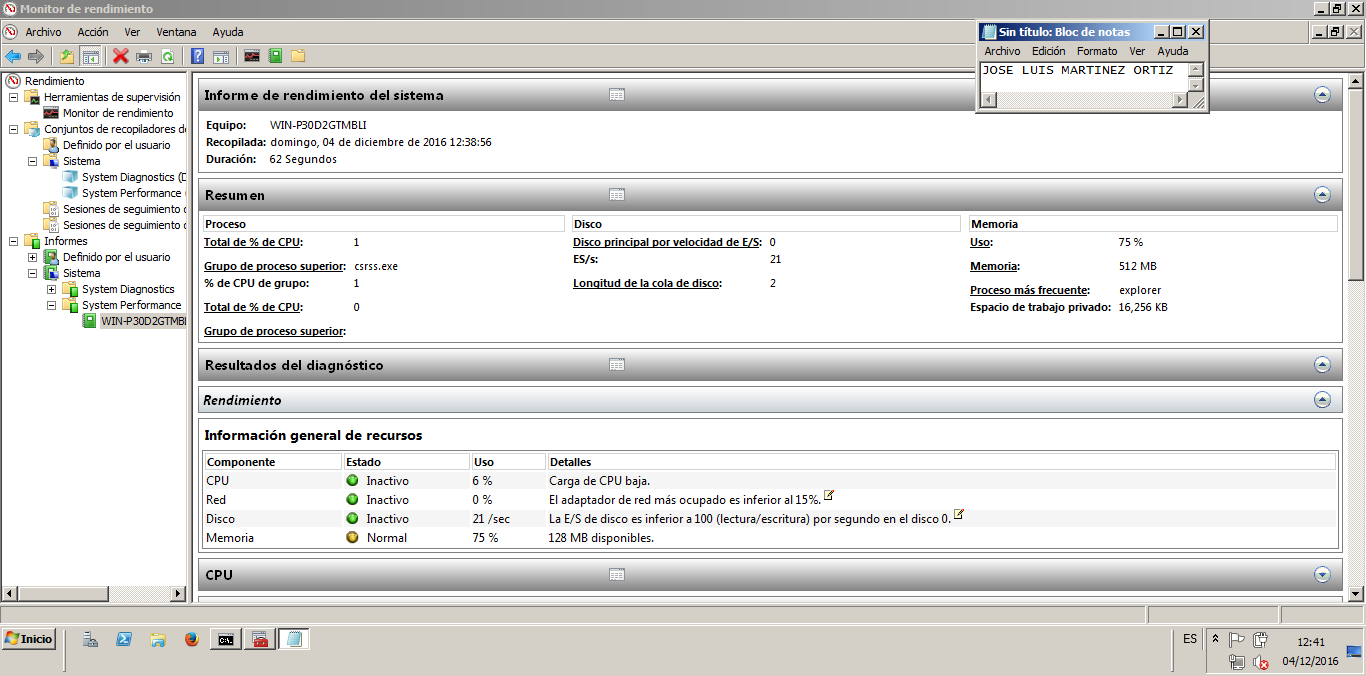
\includegraphics[scale=0.4]{./imagenes/P3_4_1.png} 
\caption{Informe del monitor de rendimiento - resumen} \label{fig:P3_4_1}
\end{figure}

\begin{figure}[H] %con el [H] le obligamos a situar aquí la figura
\centering
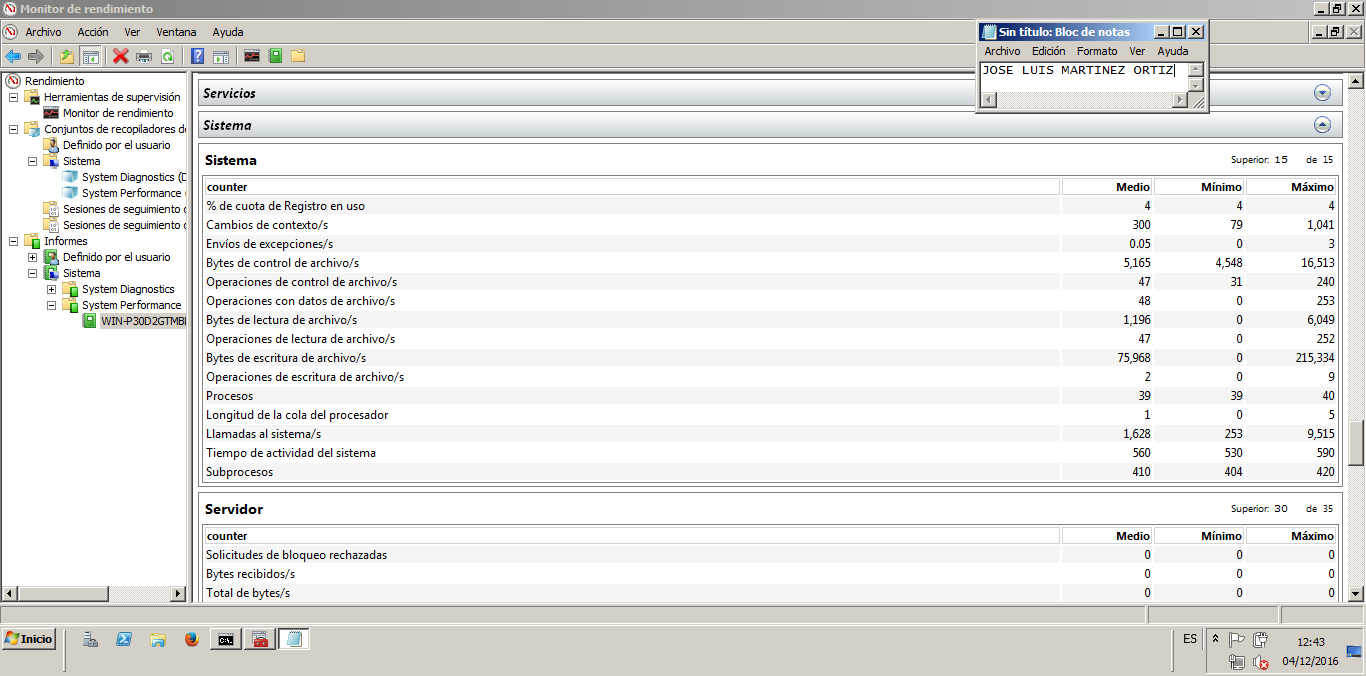
\includegraphics[scale=0.4]{./imagenes/P3_4_2.png} 
\caption{Informe del monitor de rendimiento - Sistema} \label{fig:P3_4_2}
\end{figure}

\begin{figure}[H] %con el [H] le obligamos a situar aquí la figura
\centering
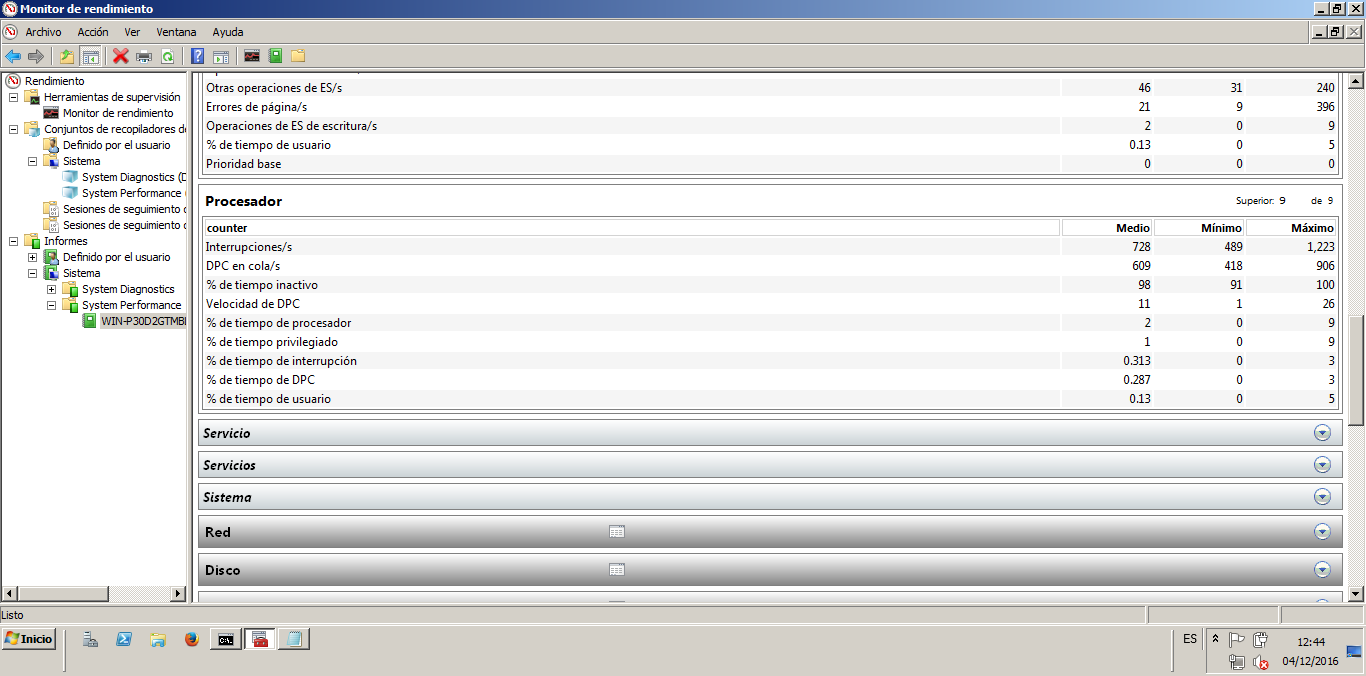
\includegraphics[scale=0.4]{./imagenes/P3_4_3.png} 
\caption{Informe del monitor de rendimiento - Procesador} \label{fig:P3_4_3}
\end{figure}

\begin{figure}[H] %con el [H] le obligamos a situar aquí la figura
\centering
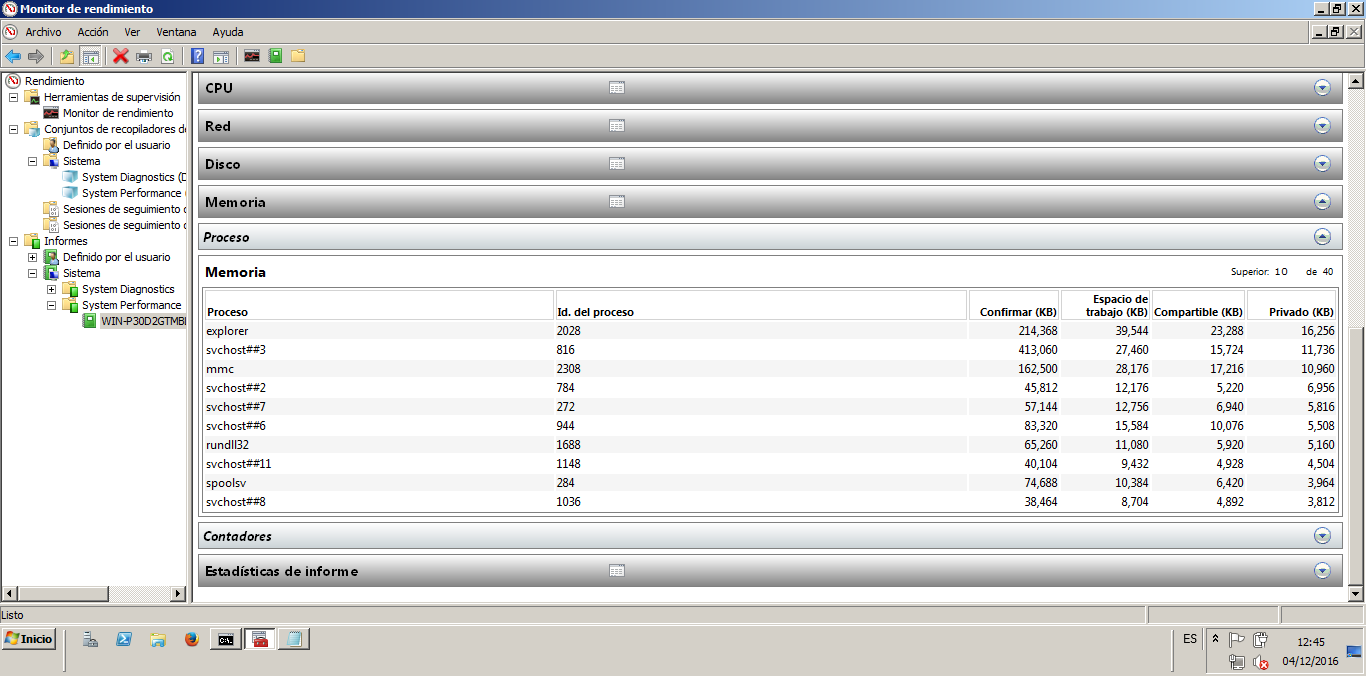
\includegraphics[scale=0.4]{./imagenes/P3_4_4.png} 
\caption{Informe del monitor de rendimiento - Memoria} \label{fig:P3_4_4}
\end{figure}
%----------------------------------------------------------------------------------------
%	Cuestión 5
%----------------------------------------------------------------------------------------

\section{Cuestión 5: Cree un recopilador de datos definido por el usuario (modo avanzado) que incluya tanto el contador de rendimiento como los datos de seguimiento: Todos los referentes al procesador, al proceso y al servicio web. Intervalo de muestra 15 segundos. Almacene el resultado en el directorio Escritorio\ logs. Incluya las capturas de pantalla de cada paso.}
Primero accedemos al programa ``\textit{perfmon}'' y seleccionamos crear un nuevo conjunto de 
recopiladores de datos. Nos aparecerá un asistente de creación (figura \ref{fig:P3_5_0}) que nos guiará
durante todo el proceso. Una vez elegida la opción de configuración manual (Avanzada) nos preguntará
que contenedores deseamos monitorizar y seleccionamos todos los de procesador, proceso y servicio web,
como se ve en la figura \ref{fig:P3_5_1}, aceptamos y seleccionamos el tiempo del intervalo a 15 segundos
(figura \ref{fig:P3_5_2}).
Por ultimo nos pedirá donde deseamos guardar la salida y elegidos Escritorio/logs (figura \ref{fig:P3_5_3}).
Y finalizamos, ahora debería aparecer el nuevo conjunto de recopiladores de datos en el Monitor de 
rendimiento, como se ve en la figura \ref{fig:P3_5_4}.



\begin{figure}[H] %con el [H] le obligamos a situar aquí la figura
\centering
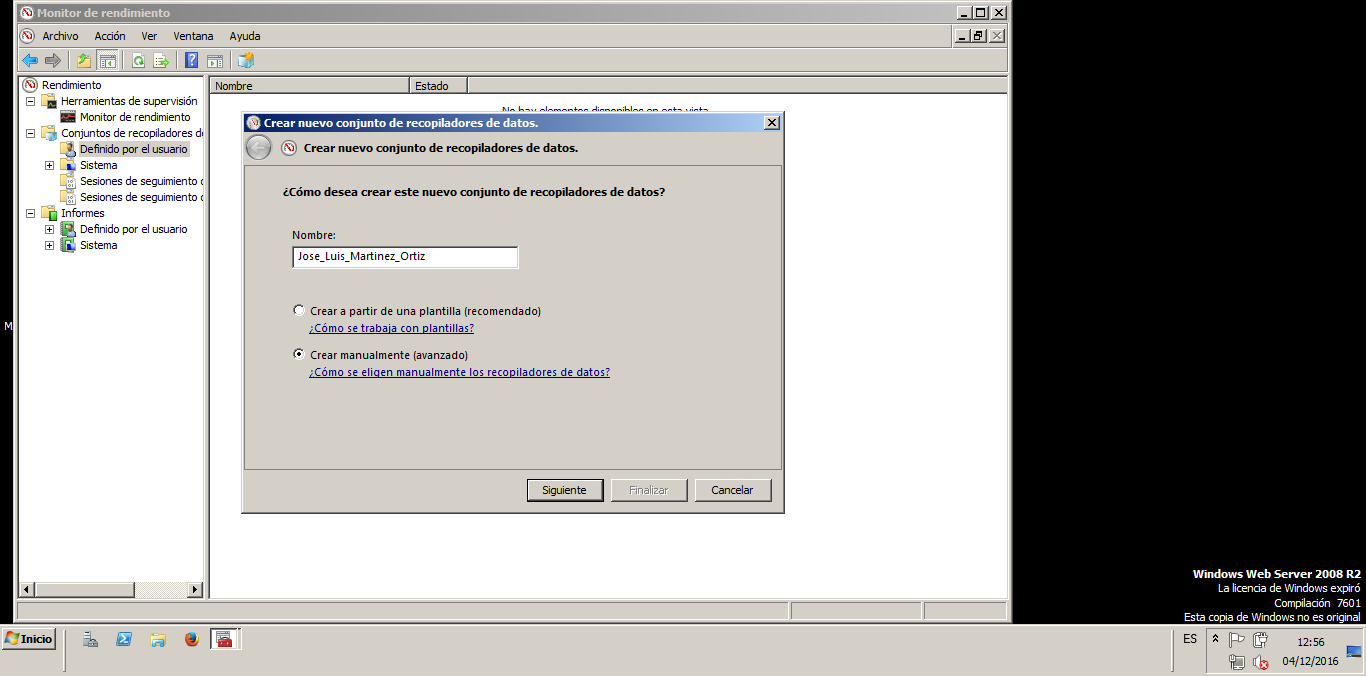
\includegraphics[scale=0.4]{./imagenes/P3_5_0.png} 
\caption{Asistente para crear un conjunto de recopilador de datos.} \label{fig:P3_5_0}
\end{figure}

\begin{figure}[H] %con el [H] le obligamos a situar aquí la figura
\centering
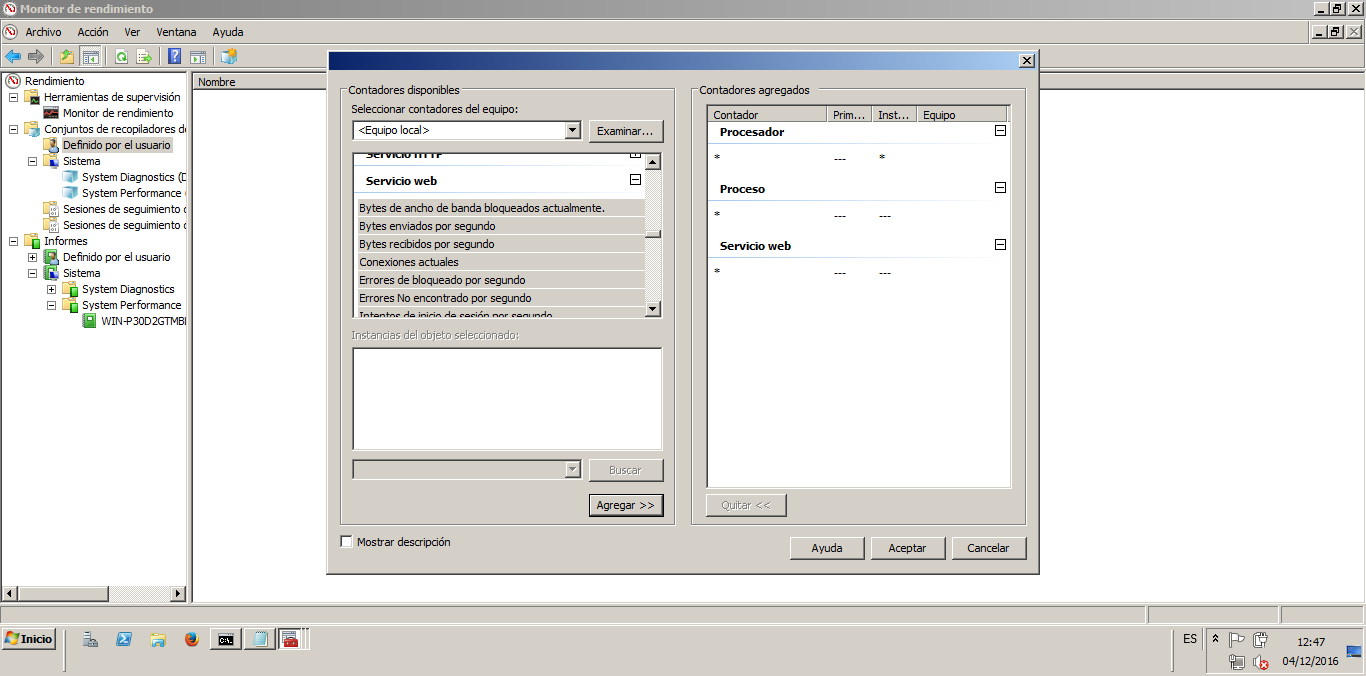
\includegraphics[scale=0.4]{./imagenes/P3_5_1.png} 
\caption{Selección de contenedores a examinar.} \label{fig:P3_5_1}
\end{figure}

\begin{figure}[H] %con el [H] le obligamos a situar aquí la figura
\centering
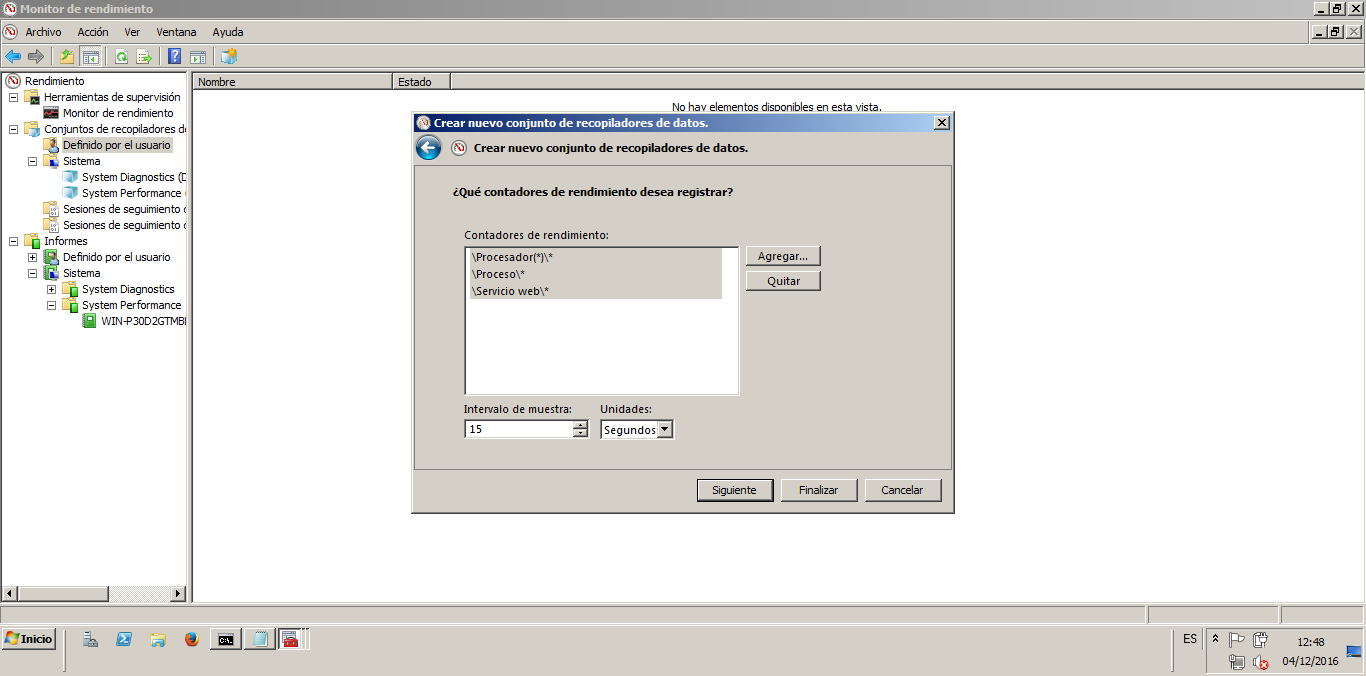
\includegraphics[scale=0.4]{./imagenes/P3_5_2.png} 
\caption{Intervalo de tiempo y contenedores a examinar.} \label{fig:P3_5_2}
\end{figure}

\begin{figure}[H] %con el [H] le obligamos a situar aquí la figura
\centering
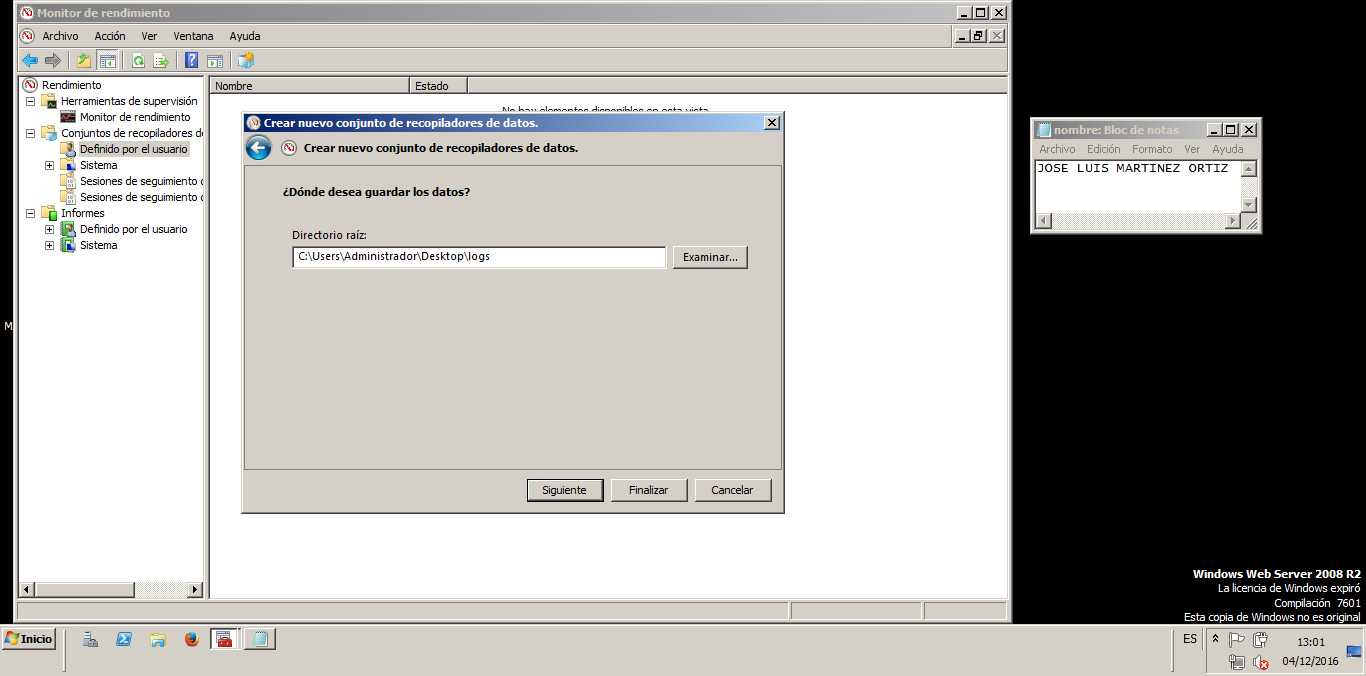
\includegraphics[scale=0.4]{./imagenes/P3_5_3.png} 
\caption{Directorio de salida de los informes.} \label{fig:P3_5_3}
\end{figure}

\begin{figure}[H] %con el [H] le obligamos a situar aquí la figura
\centering
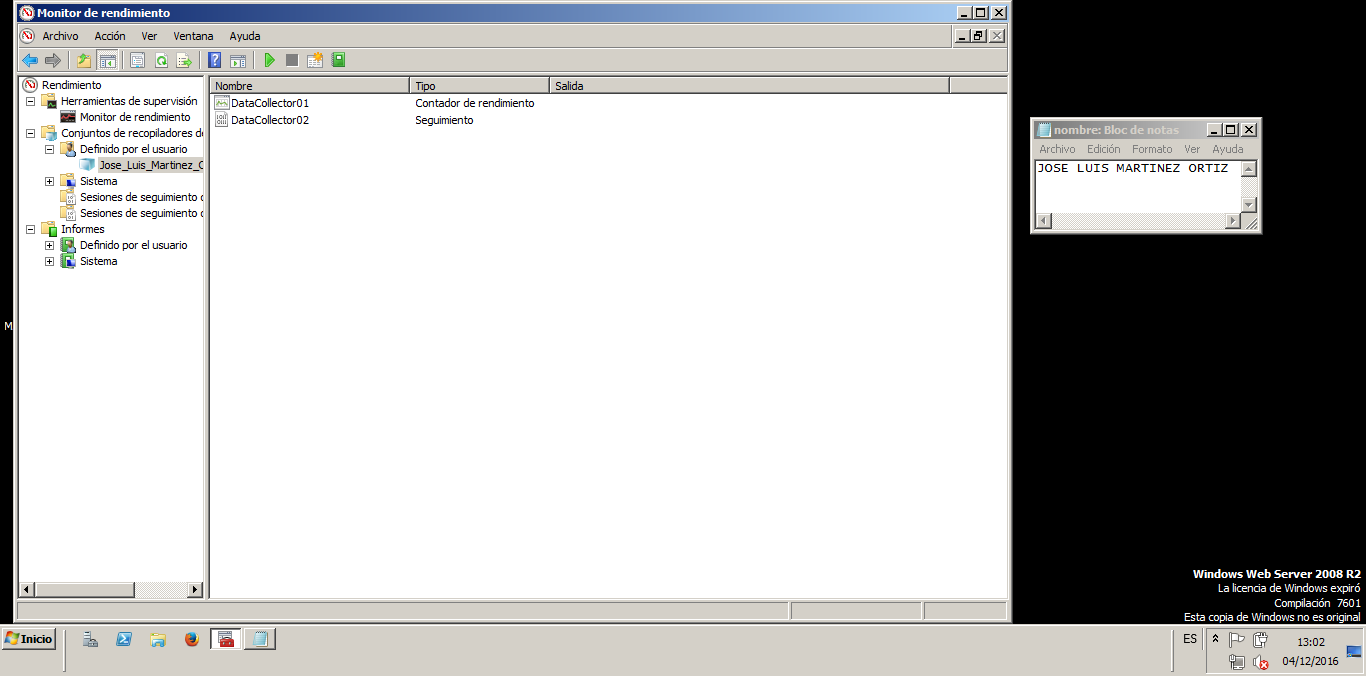
\includegraphics[scale=0.4]{./imagenes/P3_5_4.png} 
\caption{Conjunto de recopiladores de datos con el nuevo ya creado.} \label{fig:P3_5_4}
\end{figure}
%----------------------------------------------------------------------------------------
%	Cuestión 6
%----------------------------------------------------------------------------------------

\section{Cuestión 6: Visite la web del proyecto y acceda a la demo que proporcionan (http://demo.munin-monitoring.org/) donde se muestra cómo monitorizan un servidor. Monitorice varios parámetros y haga capturas de pantalla de lo que está mostrando comentando qué observa.}
En la demo de Munin hemos visto varios parámetros de monitorización entre ellos los siguientes:
\begin{itemize}
\item Monitorización de la cache. Figura \ref{fig:P3_6_1}, podemos observar como en la gráfica se 
repiten patrones, si accedemos a un zoom descubrimos que siempre hay una subida de utilización de la memoria
cache entre las 8:00 de la mañana y las 10:00. Evento razonable puesto que a primera hora del día será
cuando se empieza a utilizar el sistema y por ello tiene más accesos a cache y más fallos, dado que toda la 
noche a penas habrá estado utilizando el sistema o siempre la misma tarea.

\item Monitorización del número de Threads. Igual que pasa con la cache sobre la misma hora suele haber
una caída del número de threads en 15 aproximadamente. Esta caída habría que investigar cual es la posible
causa ya que es una caída significativa y es periódica.

\item Monitorización del Loging en el sistema. Esta vez hemos tomado una vista anual y se ve perfectamente
como a principio de Enero hay una avalancha de logins pero se va atenuando en los meses próximos hasta
prácticamente dejar de entrar al sistema, exceptuando algunos días puntuales. Una interpretación de la
gráfica sería que cuando el sistema se inicio en Enero hubo mucho transito y pruebas sobre el mismo, pero 
un mes después sobre Febrero ya se estabilizo el sistema y los accesos son puntuales para algún tipo de
mantenimiento o consultar algo esporádico.

\item Monitorización de la CPU. Aquí podemos ver que porcentaje de procesos son los que utilizan la 
CPU. En la primera figura \ref{fig:P3_6_4} vemos la monitorización de un periodo diario y otro semanal,
en la segunda figura \ref{fig:P3_6_5} vemos un periodo mensual y anual. Lo que esta claro es que el sistema
esta siempre parado, pues que el proceso ``\textit{idle}'' es el que esta prácticamente siempre ejecutándose
en todos los casos.\\
\end{itemize}
Como conclusión podemos decir que el sistema se inició el Enero y cuenta con un hardware muy por encima de lo
que realmente esta siendo usado, por lo que a habido una mala elección del Sistema para el uso que se 
le esta haciendo. Otra posibilidad es que el sistema se pensara para un escenario pero dicho escenario
 no se ha producido por falta de clientes/trabajos al sistema.

\begin{figure}[H] %con el [H] le obligamos a situar aquí la figura
\centering
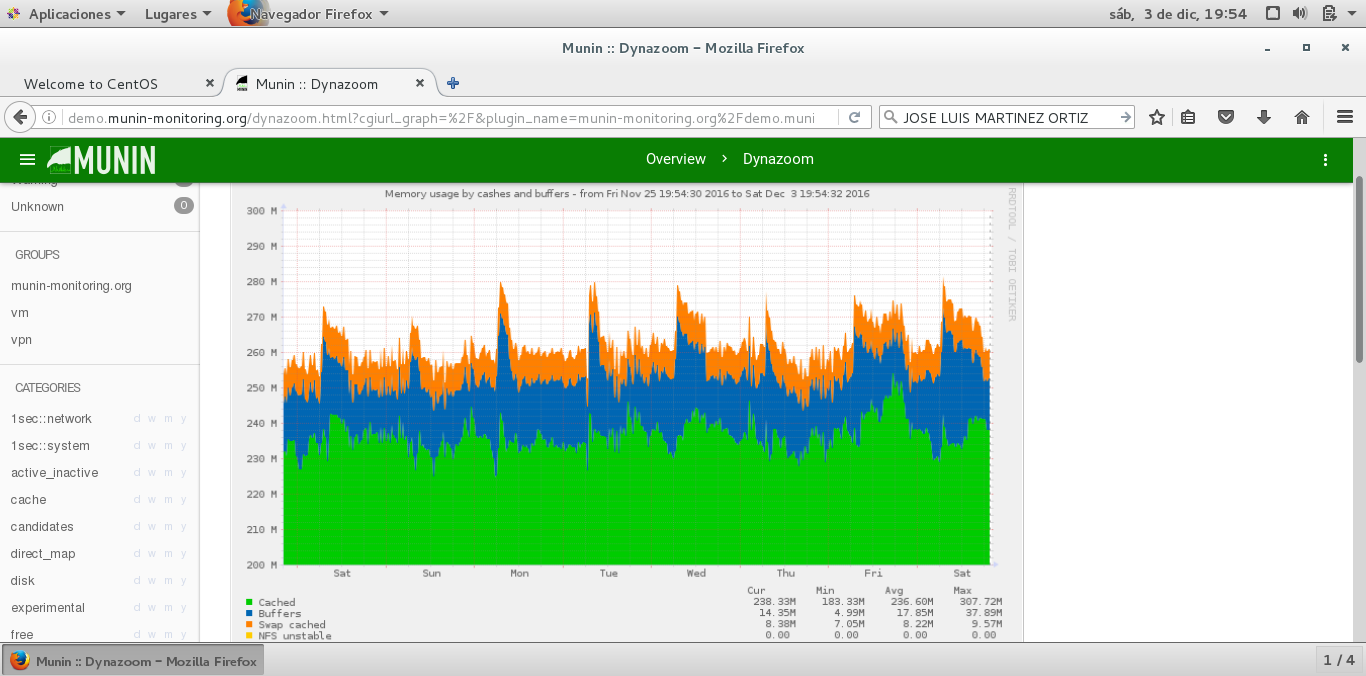
\includegraphics[scale=0.4]{./imagenes/P3_6_1.png} 
\caption{Munin, monitorización de la cache del sistema} \label{fig:P3_6_1}
\end{figure}

\begin{figure}[H] %con el [H] le obligamos a situar aquí la figura
\centering
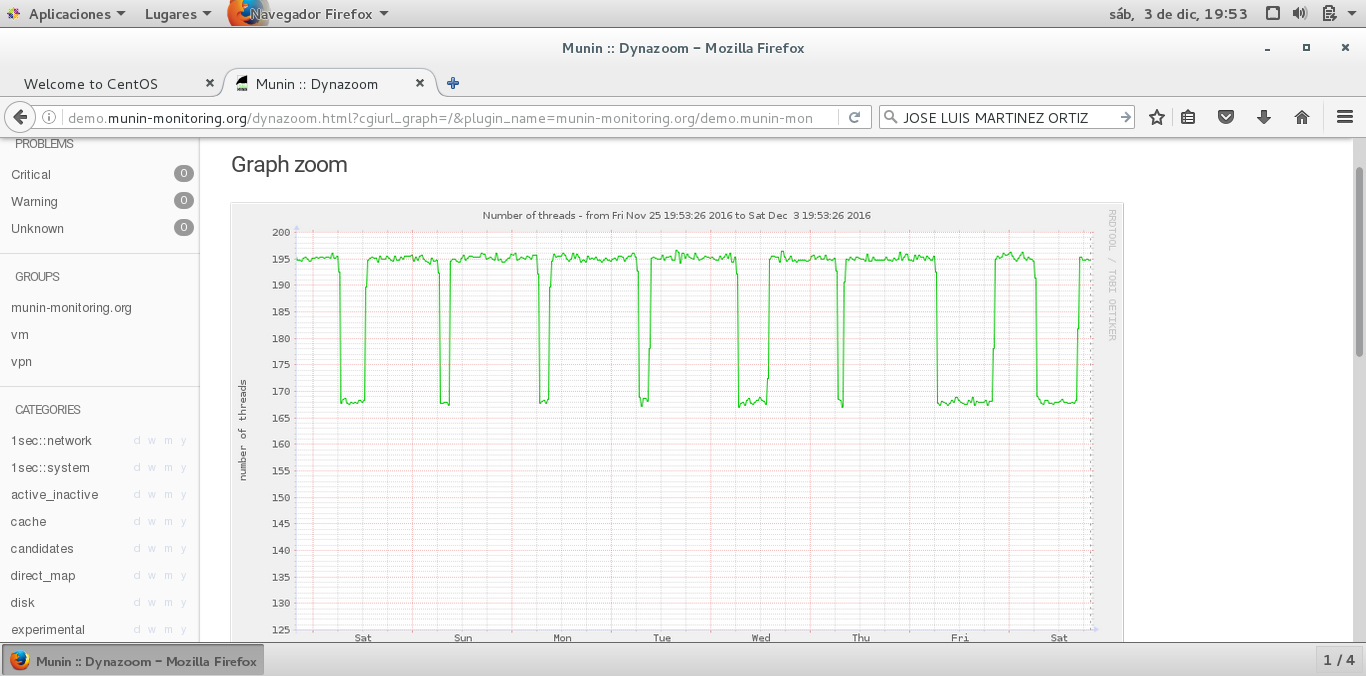
\includegraphics[scale=0.4]{./imagenes/P3_6_2.png} 
\caption{Munin, monitorización del número de Threads} \label{fig:P3_6_2}
\end{figure}

\begin{figure}[H] %con el [H] le obligamos a situar aquí la figura
\centering
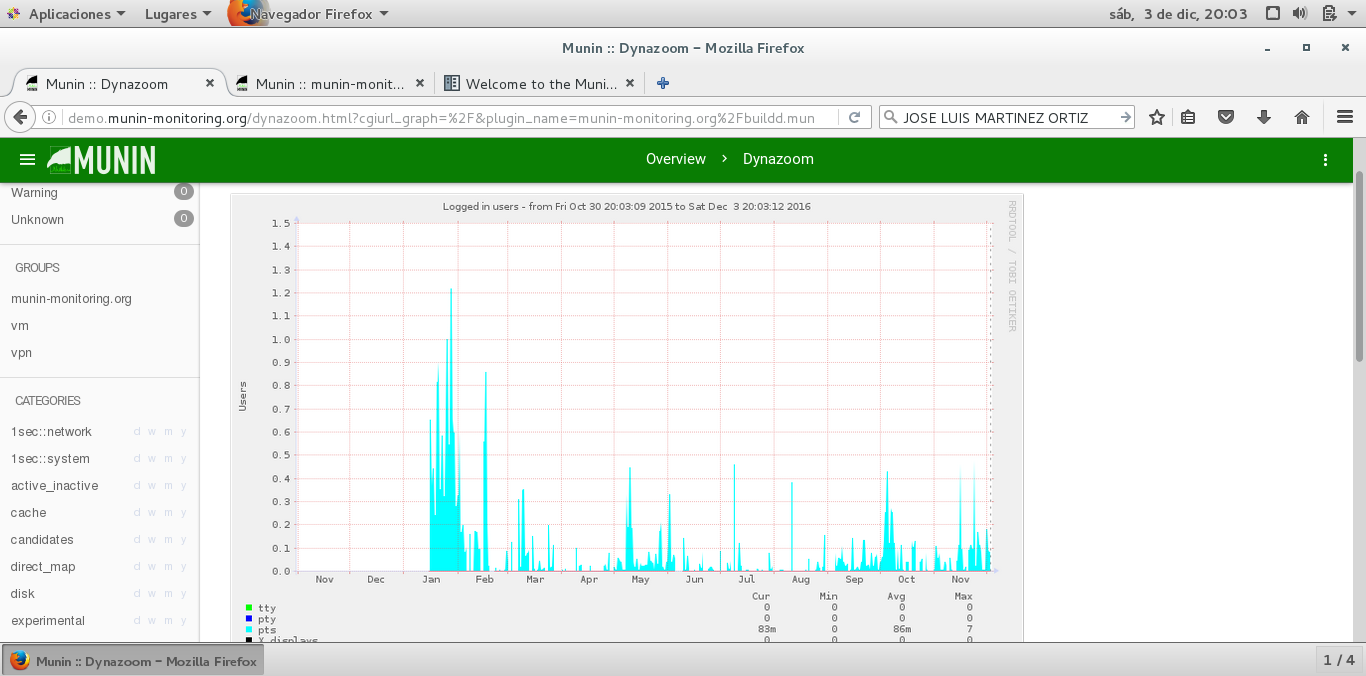
\includegraphics[scale=0.4]{./imagenes/P3_6_3.png} 
\caption{Munin, monitorización del número de login al sistema} \label{fig:P3_6_3}
\end{figure}

\begin{figure}[H] %con el [H] le obligamos a situar aquí la figura
\centering
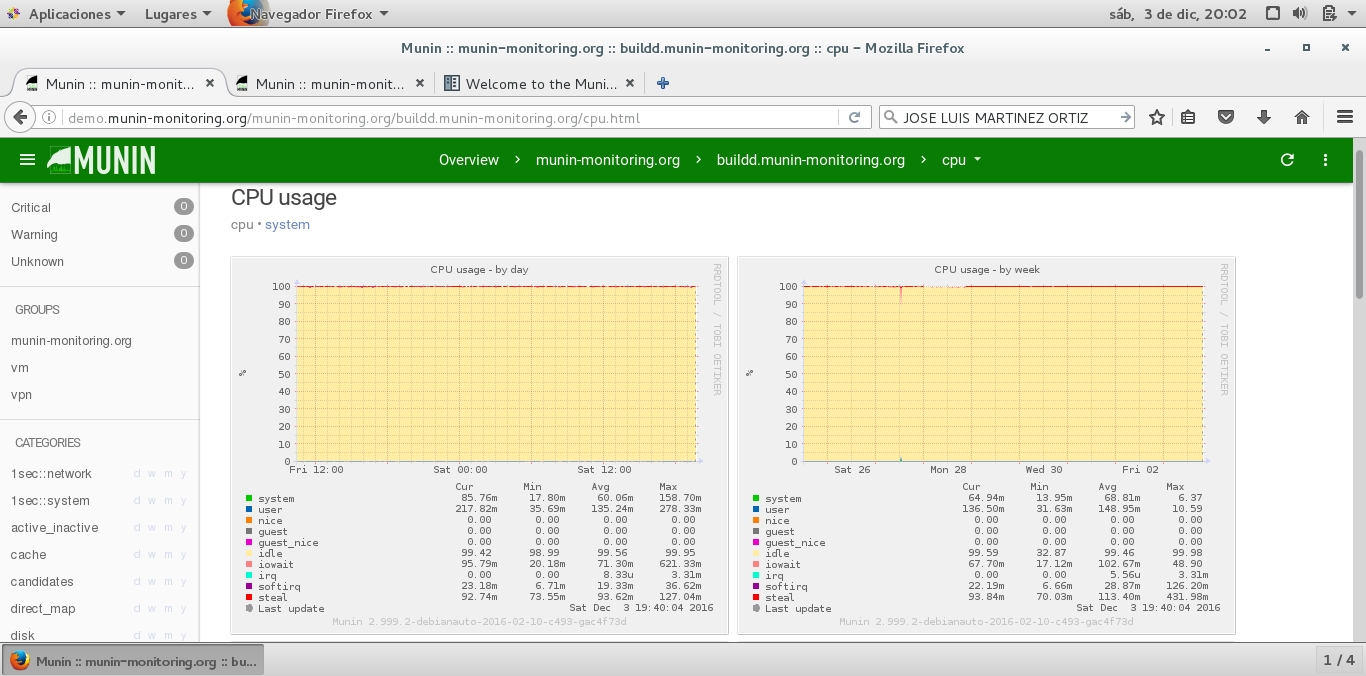
\includegraphics[scale=0.4]{./imagenes/P3_6_4.png} 
\caption{Munin, monitorización de la cpu} \label{fig:P3_6_4}
\end{figure}

\begin{figure}[H] %con el [H] le obligamos a situar aquí la figura
\centering
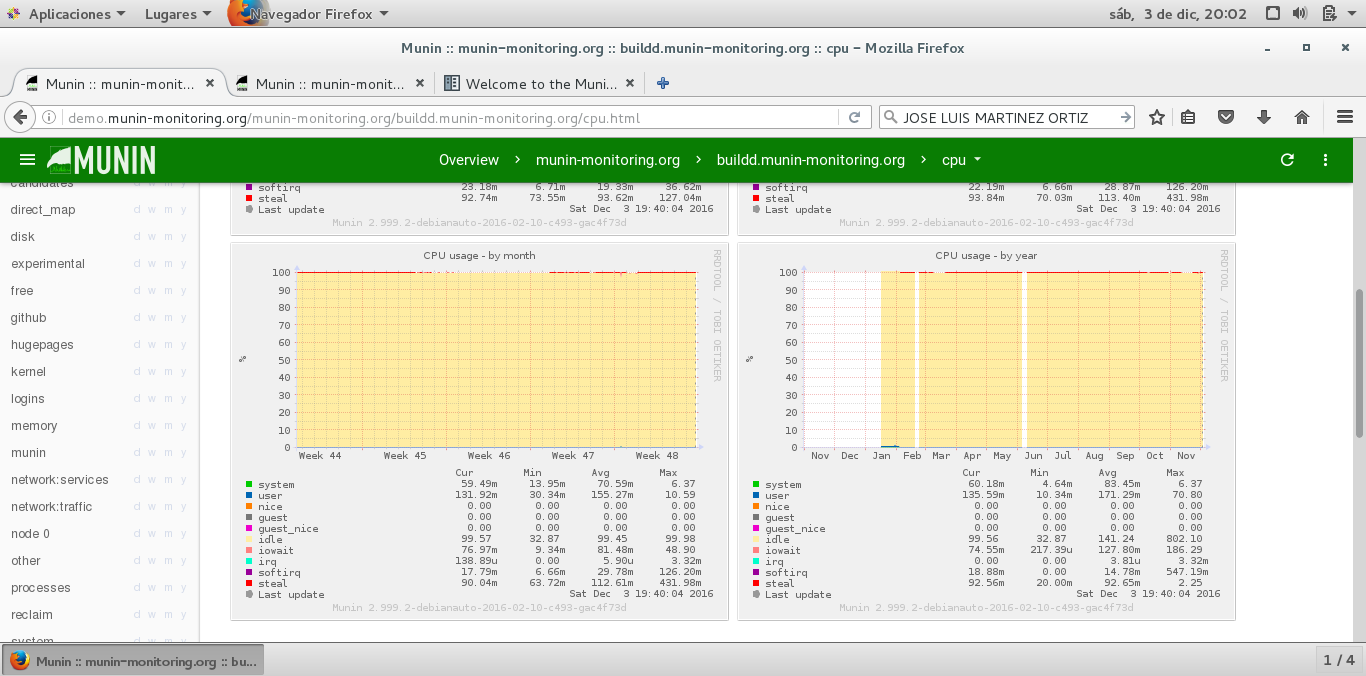
\includegraphics[scale=0.4]{./imagenes/P3_6_5.png} 
\caption{Munin, monitorización de la cpu} \label{fig:P3_6_5}
\end{figure}



%----------------------------------------------------------------------------------------
%	Cuestión 7
%----------------------------------------------------------------------------------------

\section{Cuestión 7: Escriba un breve resumen sobre alguno de los artículos donde se muestra el uso de strace o busque otro y coméntelo.}
Voy a comentar y resumir el caso de \textit{Chad Fowler}, quien resolvió un problema sobre e acceso a unos ficheros de 
la base de datos que no dejaba acceder a ellos, el cual resolvió con
 \texttt{Strace}. Primero ejecuto un ``\textit{Hola}'' en C con \textit{Strace}.
Para ver todo el proceso de llamadas al sistema que realizaba su ejecución
y descubrió que al principio se llama a \textit{execve()} y al final se
llamaba a \textit{write()} con el mensaje a mostrar. Pero entre medias 
había muchas llamadas necesarias para la ejecución de programas. Ahora 
tenia que ver el trazado real del programa que contenía el problema.
Empieza mirando las primeras lineas y descubre que utiliza la llamada
\textit{select()} para conseguir los descriptores de archivo de entrada
y salida de su programa, después de mirar un poco mas en profundidad 
determina que es correcto el uso del \textit{select()} ya que utiliza 
\textit{socket} para entrada y salida. Continuando el análisis descubre
un trozo realmente interesante, una llamada a \textit{recvfrom()} donde
puede ver el mensaje HTTP que se envía perfectamente, pero sin nada fuera
de lo normal. Siguiendo la trazada se realizan varias llamadas para comprobar
 datos de los sockets hasta que realiza una llamada a una Base de Datos
 externa y se para a analizar su contenido. 
  Acaba el análisis de \textit{Strace} 
 sin nada fuera de lo normal, por ello ahora vuelve a lanzar \textit{Strace}
 pero con el flag ``-c'' para ver el número de llamadas que realiza.
 Siguió examinando la trazada y obtuvo una ``pista'' como Chad indica. La 
 pista fue que el sistema iba lento cuando realizaban llamadas con ``\textit{sudo}'' por lo que siguieron esta linea hasta que los llevo a descubrir
 que en la declaración del registro se encontraba el problema de la lentitud.
 Con lo que pudieron centrarse en ese foco para solucionar el problema y 
 todo gracias al seguimiento que hace \textit{Strace} de un programa.
 

%----------------------------------------------------------------------------------------
%	Cuestión 8
%----------------------------------------------------------------------------------------

\section{Cuestión 8: Escriba un script en Python o PHP y analice su comportamiento usando el profiler presentado.}
Utilizo un Script en Python que encuentra los números primos entre un rango, pongo un rango bastante
grande para que el script dure un rato y así poder ver bien. En la figura \ref{fig:P3_8_2} se puede ver
el contenido del Script. Lanzamos el Script con la opción del profiler ``\textit{cProfiler}'', 
figura \ref{fig:P3_8_1} y observamos la salida que nos muestra. Con la ayuda de la 
documentación \cite{CProfiler} entendemos que significa esa salida.
Podemos concluir que se ha realizado una única llamada al script y el cual ha tardado 67.445 segundos
excluyendo llamadas externas y que en total ha tardado 89.847 segundos en ejecutar el script. El
profiler de Python es muy útil para averiguar el tiempo que tarda cada función del script y así 
saber por ejemplo que función es la que mas ocupa y poder optimizarla.



\begin{figure}[H] %con el [H] le obligamos a situar aquí la figura
\centering
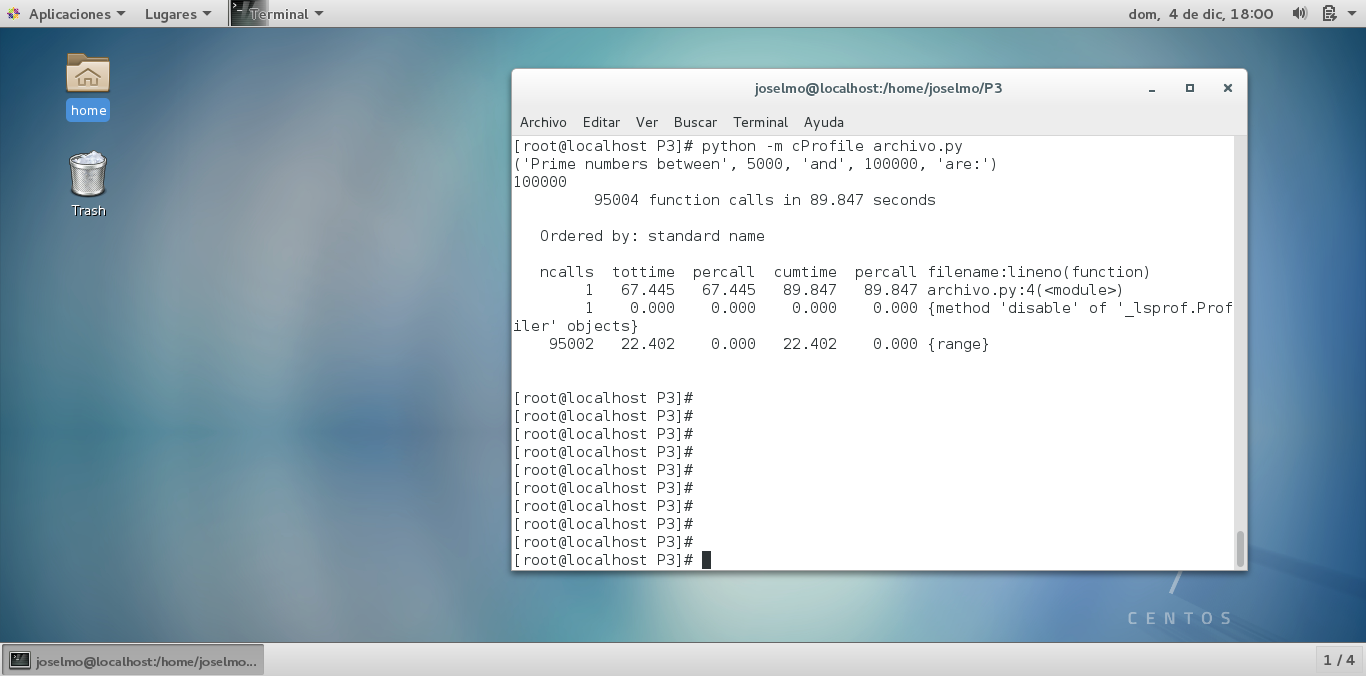
\includegraphics[scale=0.4]{./imagenes/P3_8_1.png} 
\caption{Script en Python para calcular números primos.} \label{fig:P3_8_1}
\end{figure}

\begin{figure}[H] %con el [H] le obligamos a situar aquí la figura
\centering
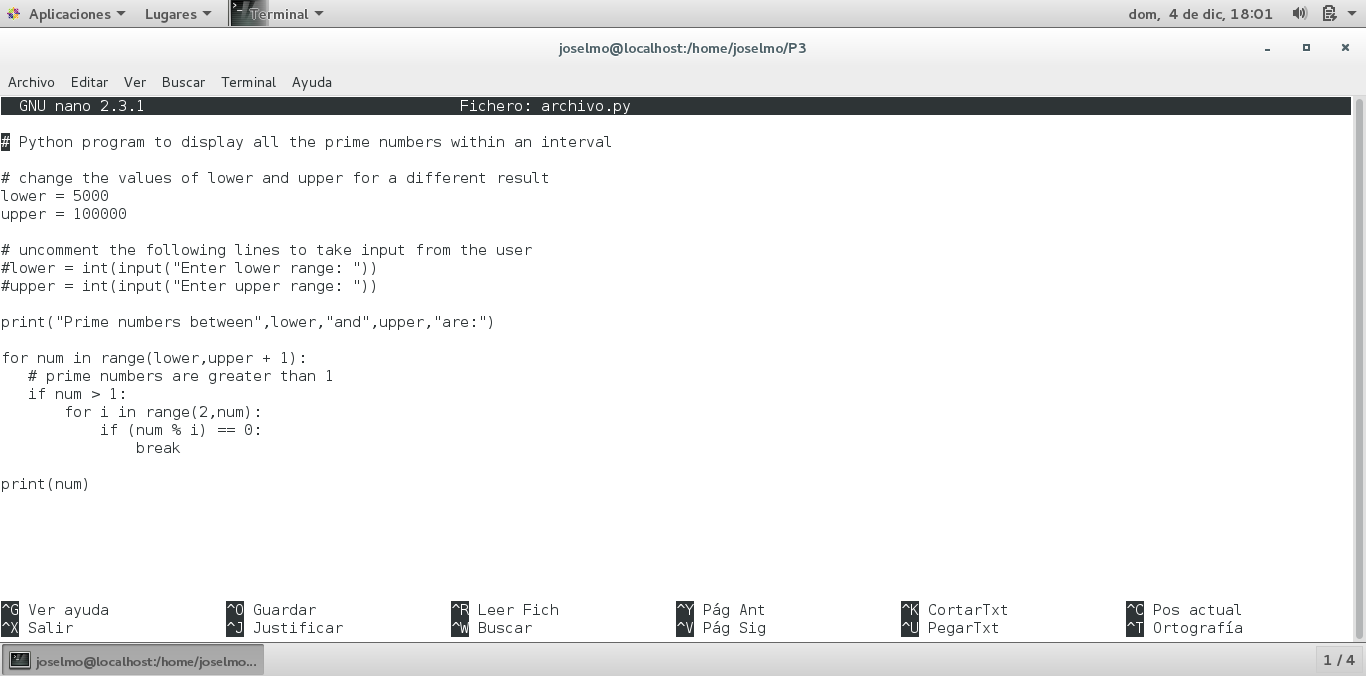
\includegraphics[scale=0.4]{./imagenes/P3_8_2.png} 
\caption{Ejecución del script de Python con el CProfiler activado.} \label{fig:P3_8_2}
\end{figure}



%----------------------------------------------------------------------------------------
%	Cuestión 9 
%----------------------------------------------------------------------------------------

\section{Cuestión 9: Acceda a la consola mysql (o a través de phpMyAdmin) y
muestre el resultado de mostrar el ``profile'' de una consulta (la creación de
la BD y la consulta la puede hacer libremente).}
Realizamos una conexión a la base de datos ``\textit{Restaurante}'' una de prueba, 
figura \ref{fig:P3_9_1}, comprobamos cuantos profiler hay ya definidos con el comando 
\texttt{select @@profiling} vemos que hay cero por lo tanto vamos a crearnos unos con
 el comando \texttt{set profiling = 1} y pasamos a crear una tabla nueva, pero ya existe
 por lo que la borramos y volvemos a crear la tabla (figura \ref{fig:P3_9_2}). Ahora consultamos
 los profiler que hay creado y vemos que existen 3, una por cada interacción con la base de datos.
Le indicamos que queremos ver el profiling primero (figura \ref{fig:P3_9_3}) y observamos el tiempo
de duración de cada sub-tarea que ha necesitado la llamada a la base de datos para crear la tabla ``T1''  


\begin{figure}[H] %con el [H] le obligamos a situar aquí la figura
\centering
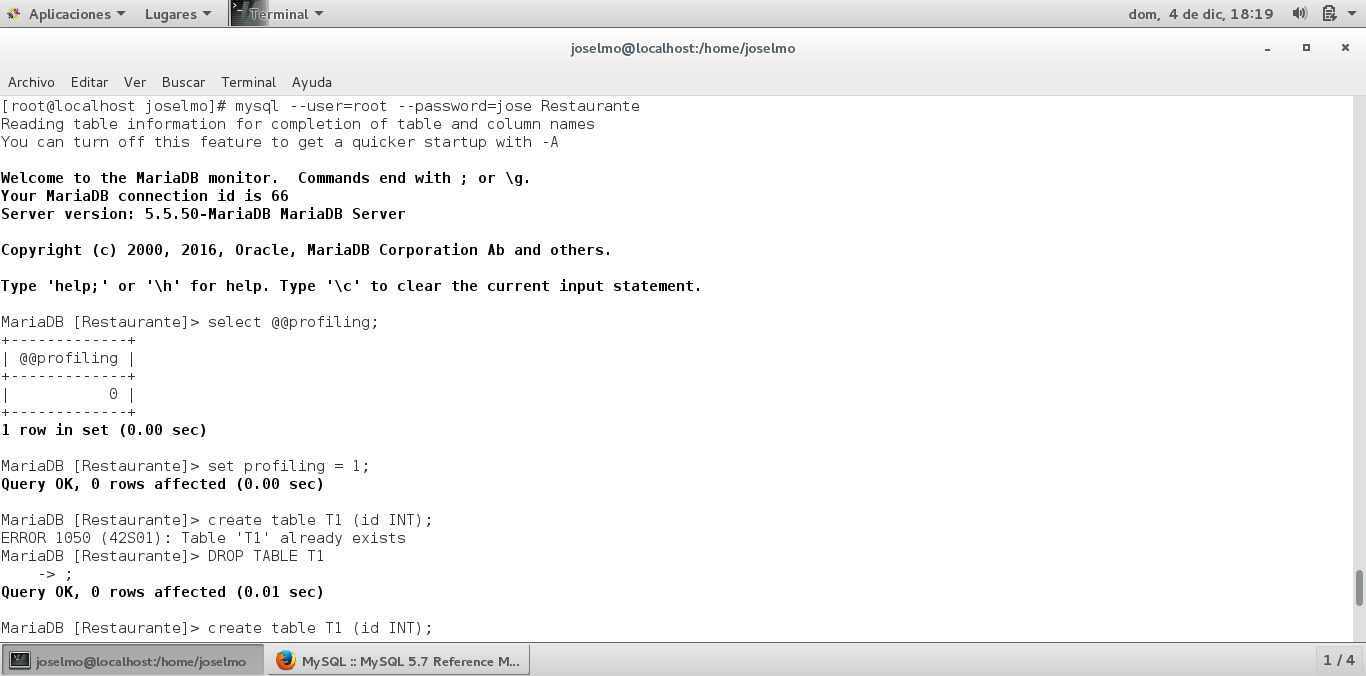
\includegraphics[scale=0.4]{./imagenes/P3_9_1.png} 
\caption{MySQL } \label{fig:P3_9_1}
\end{figure}

\begin{figure}[H] %con el [H] le obligamos a situar aquí la figura
\centering
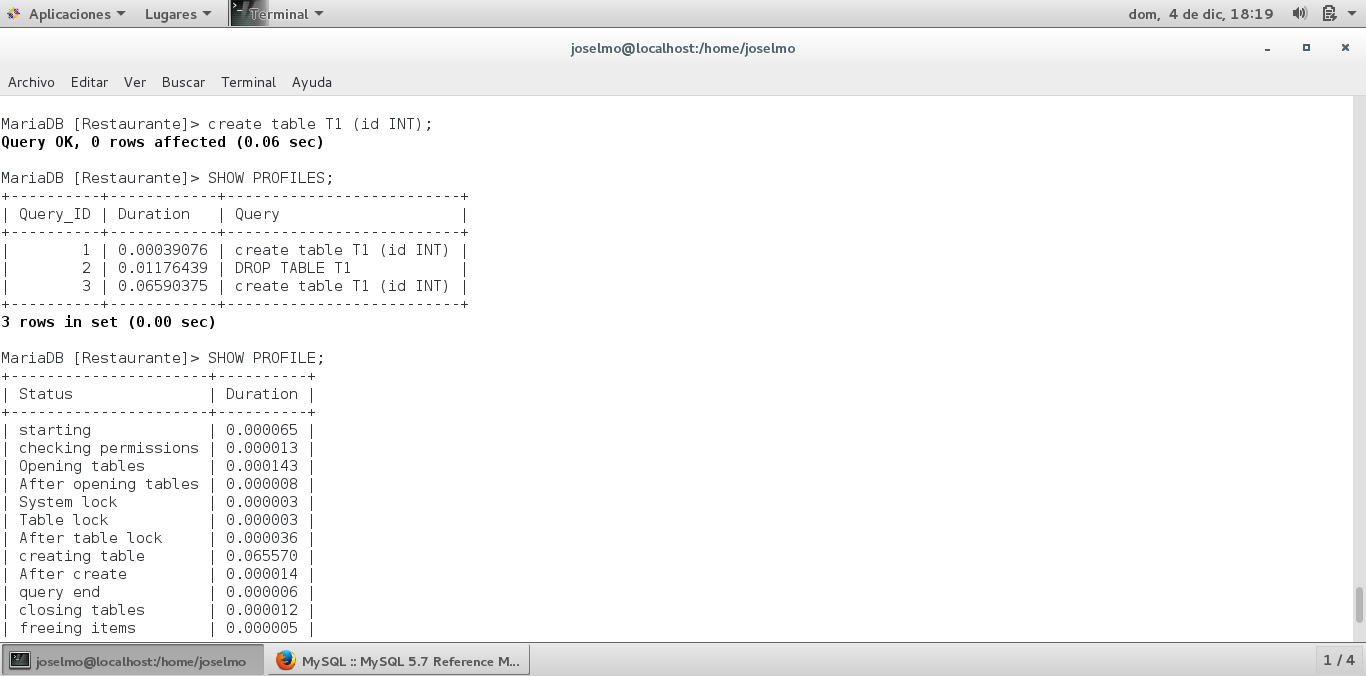
\includegraphics[scale=0.4]{./imagenes/P3_9_2.png} 
\caption{MySQL } \label{fig:P3_9_2}
\end{figure}

\begin{figure}[H] %con el [H] le obligamos a situar aquí la figura
\centering
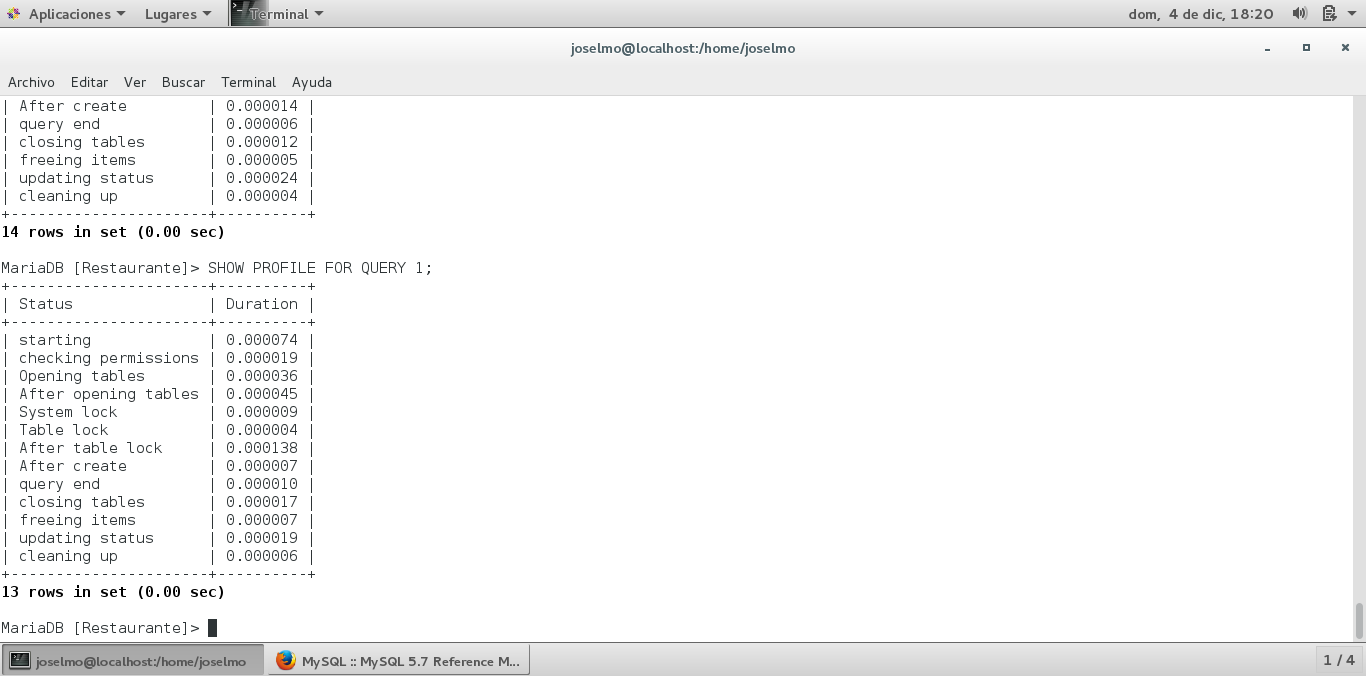
\includegraphics[scale=0.4]{./imagenes/P3_9_3.png} 
\caption{MySQL } \label{fig:P3_9_3}
\end{figure}



%----------------------------------------------------------------------------------------
%	Tareas extra
%----------------------------------------------------------------------------------------
\section{Tareas extra.}
\subsection{Problema de la red ``Red NAT'' de VirtualBox}
VirtualBox utilizado: \textit{Versión 5.1.10 r112026 (Qt5.5.1)}
Sistema Operativo:	\textit{Ubuntu Desktop 16.04}
Máquina:	\textit{asus-k55mv}

La red NAT de virtualbox contempla la posibilidad de conectar internamente todas las máquinas virtuales
de la red y además ofrece la posibilidad de conexión a internet con una IP propia de cada máquina virtual.
Para crear una red NAT he utilizado tanto la interfaz gráfica que provee VirtualBox como la terminal
de comandos con \textit{VBoxManage}. Con ambas redes configuradas en las máquinas virtuales de CentOS y
Ubuntu Server comprobamos que la conexión entre ellas funciona correctamente, pero a la hora de 
conectarse a internet no funciona. El fallo es conocido como se recoge en la web del seguimiento de Bugs
de VirtualBox y el motivo es que las redes "Red NAT" creadas no las guarda como natnet, tipo de redes "RED NAT"
, con lo que no funciona este tipo de red en esta versión de VirtualBox.


\begin{figure}[H] %con el [H] le obligamos a situar aquí la figura
\centering
%\includegraphics[scale=0.5]{./imagenes/P2_10_host_2.png}  %el parámetro scale permite agrandar o achicar la imagen. En el nombre de archivo puede especificar directorios
\caption{Configuración de VirtualBox} \label{fig:P3_T1_1}
\end{figure}

\subsection{Instalación y utilización de lm-sensors}
Para probar el software que se indica en el guión de prácticas \textit{lm-sensor} consulto 
la wiki de Arch \cite{lmSensor}, ya que la web indicada en el guión no esta operativa.
Lo realizo sobre mi propio equipo ya que en las máquinas virtuales no cuentan con los sensores de
las BIOS.
Como se puede ver en la imagen \ref{fig:P3_E2_1} ya tengo instalado el software. Ahora paso a 
configurar a que sensores de mi equipo le doy acceso para monitorizar (figura \ref{fig:P3_E2_2}).
Una vez configurado los permisos ya podemos ver la información mediante el comando \textit{sensors},
tal como se ve en la figura \ref{fig:P3_E2_3}.\\

Podemos ver como la temperatura de los ``cores'' esta en valores normales, además nos indica que por
encima de 81º es una temperatura alta y por encima de los 105º ya es critica. También nos informa de la
velocidad del ventilador del equipo, en nuestro caso esta funcionando a 27000 rpm (revoluciones por minuto)

\begin{figure}[H] %con el [H] le obligamos a situar aquí la figura
\centering
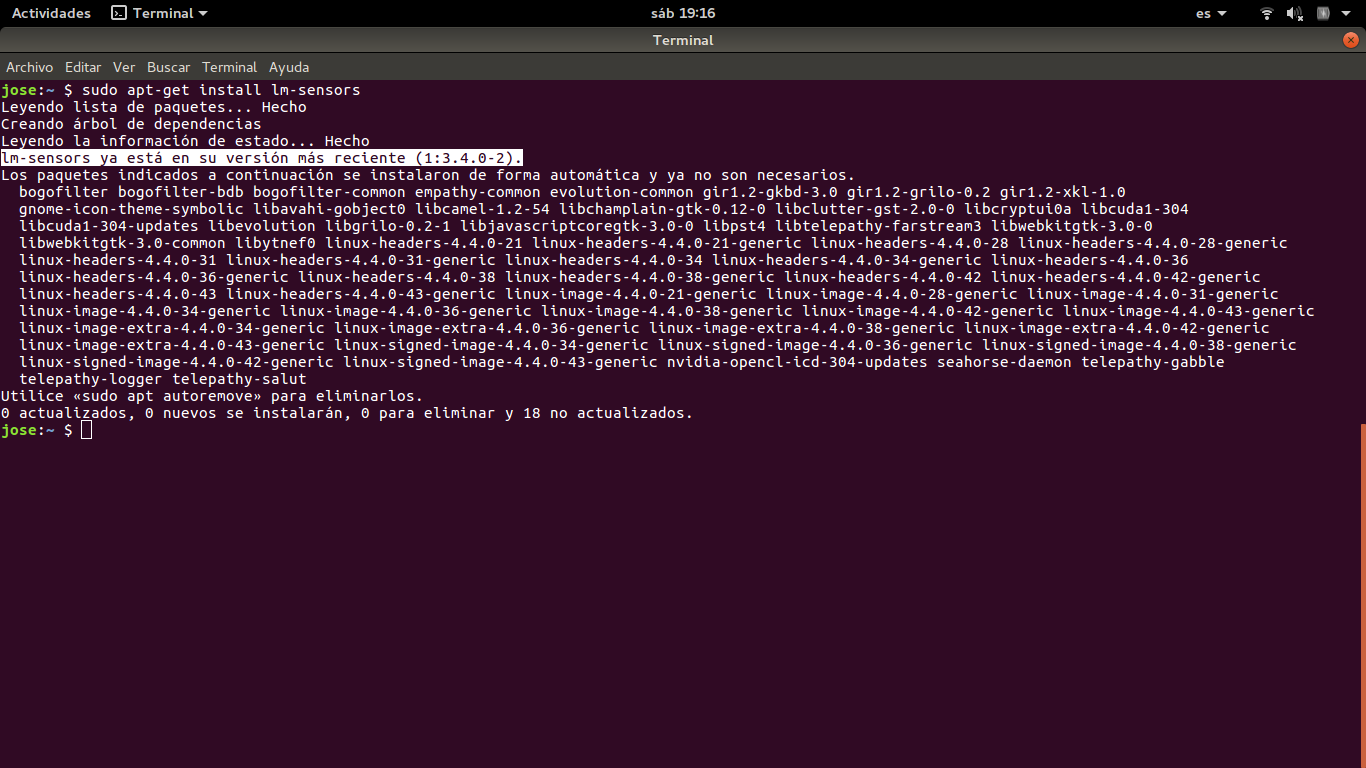
\includegraphics[scale=0.3]{./imagenes/P3_E2_1.png}  %el parámetro scale permite agrandar o achicar la imagen. En el nombre de archivo puede especificar directorios
\caption{Instalación de lm-sensors} \label{fig:P3_E2_1}
\end{figure}

\begin{figure}[H] %con el [H] le obligamos a situar aquí la figura
\centering
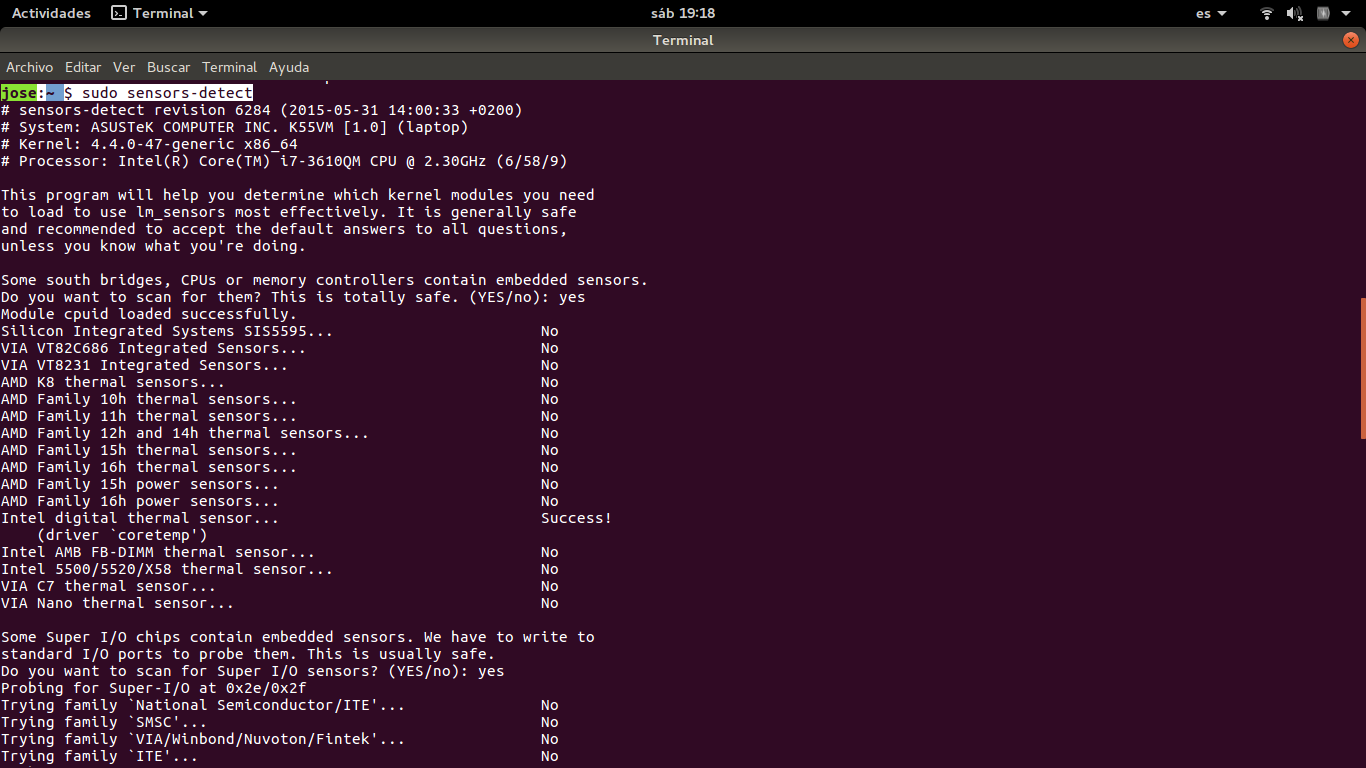
\includegraphics[scale=0.3]{./imagenes/P3_E2_2.png}  %el parámetro scale permite agrandar o achicar la imagen. En el nombre de archivo puede especificar directorios
\caption{Configuración de lm-sensors} \label{fig:P3_E2_2}
\end{figure}

\begin{figure}[H] %con el [H] le obligamos a situar aquí la figura
\centering
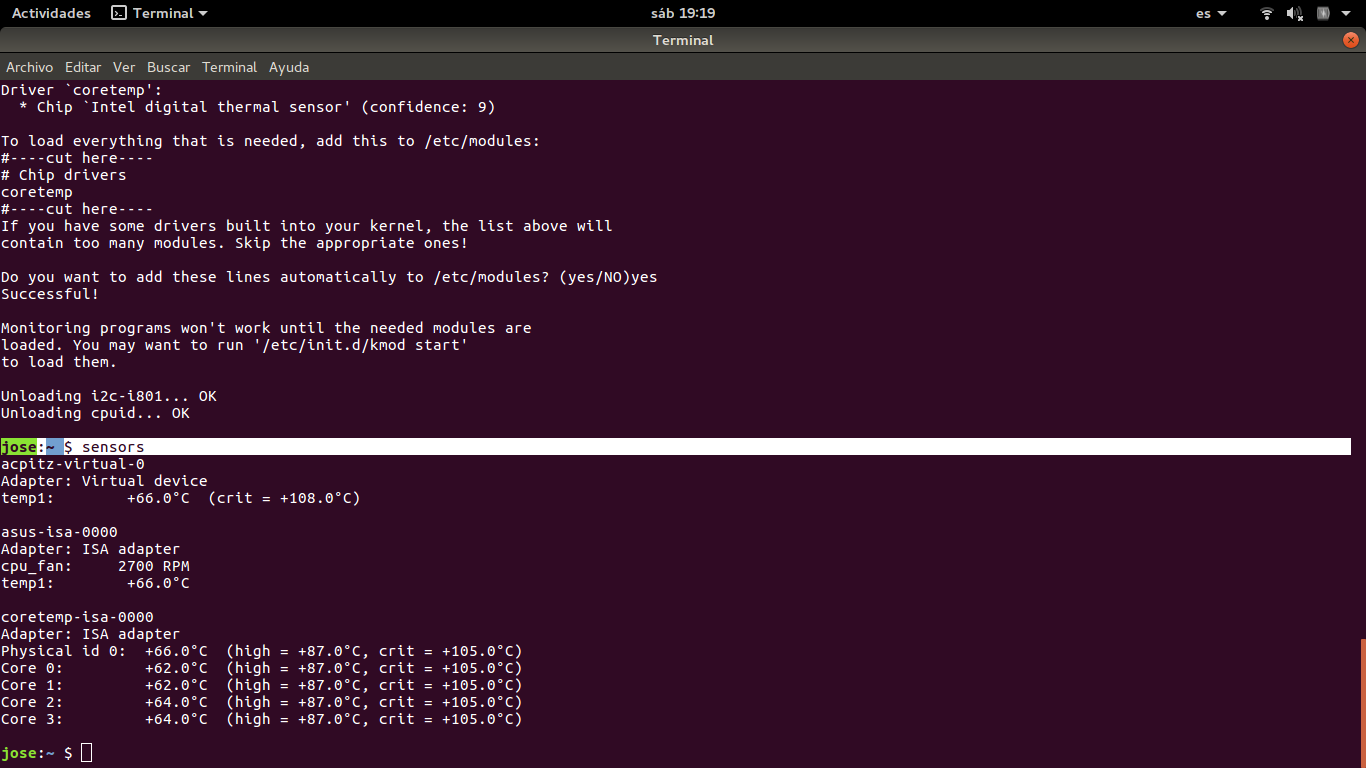
\includegraphics[scale=0.3]{./imagenes/P3_E2_3.png}  %el parámetro scale permite agrandar o achicar la imagen. En el nombre de archivo puede especificar directorios
\caption{Salida de lm-sensors} \label{fig:P3_E2_3}
\end{figure}



%------------------------------------------------

\bibliography{citas} %archivo citas.bib que contiene las entradas 
\bibliographystyle{plain} % hay varias formas de citar

\end{document}



